\subsection{备忘录模式(Memento)}

\subsubsection{备忘录模式简介}

备忘录模式是一种行为型设计模式,它提供了一种方法来保存一个对象的内部状态,并在需要时可以将对象恢复到之前保存的状态。

备忘录模式的实现包括三个部分:

发起人类:发起人类是一个需要保存内部状态的类,它可以创建一个备忘录来保存当前的内部状态,并在需要时通过备忘录恢复先前的内部状态。

备忘录类:备忘录类是一个负责保存发起人类内部状态的类,它可以通过一个对象来保存发起人类的内部状态,并在需要时返回这个对象,以便发起人类恢复先前的状态。

管理者类:管理者类是一个负责管理备忘录的类,它可以保存多个备忘录,并可以提供撤销和恢复的功能,以便发起人类可以方便地撤销和恢复先前的操作。

备忘录模式具有以下优点:

可以保存对象的内部状态,并在需要时将对象恢复到先前保存的状态,从而实现对撤销和恢复操作的支持。

可以将备忘录作为一个独立的对象进行管理,从而避免发起人类过于臃肿,并提高了系统的可维护性和可扩展性。

可以通过管理者类来管理备忘录,从而提高了系统的可控性。

同时,备忘录模式也有一些缺点:

备忘录对象需要占用一定的内存空间,因此在某些情况下可能会导致内存开销增大。

备忘录模式需要为每个需要支持撤销和恢复操作的类定义一个与其对应的备忘录类。

\subsubsection{备忘录模式在项目中的应用}

\begin{figure}[h]
  \centering
  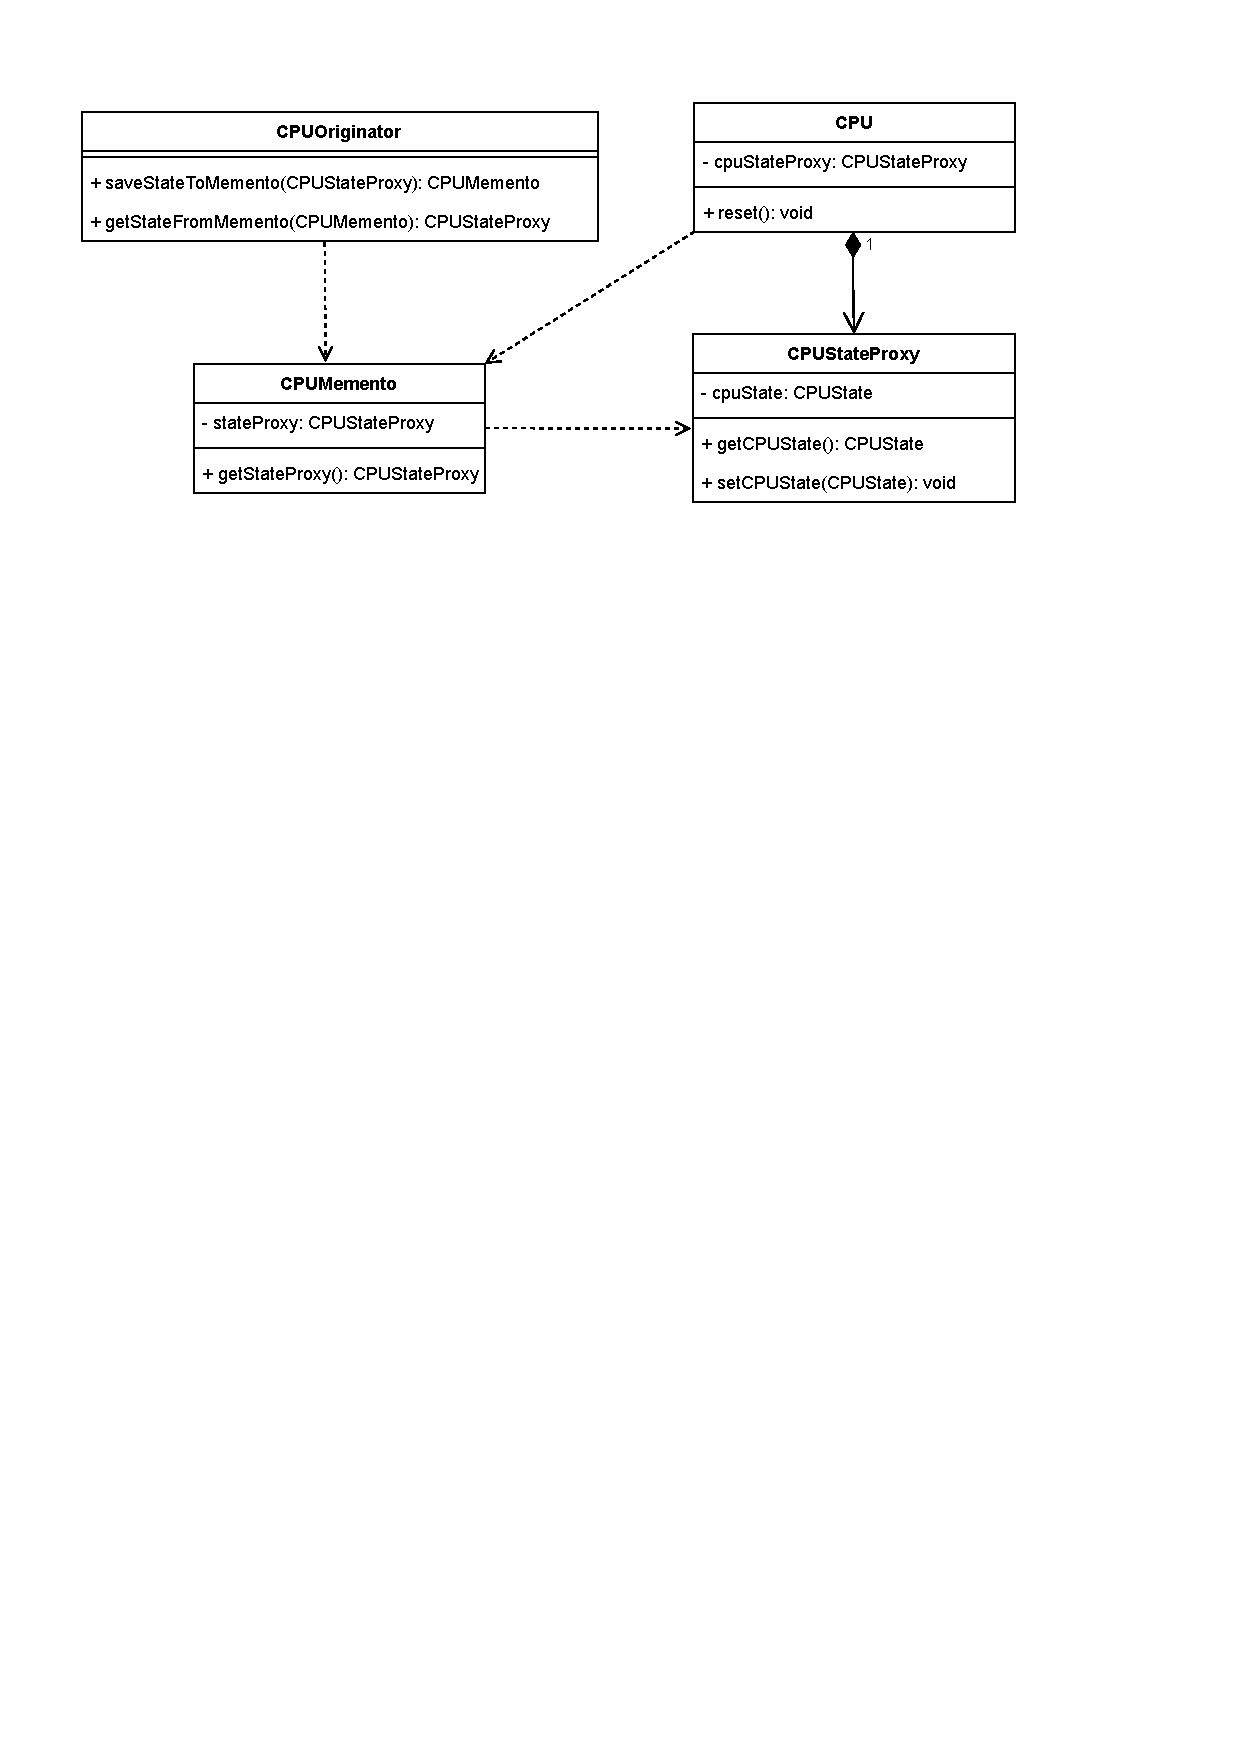
\includegraphics[width=0.9\textwidth]{figures/备忘录.pdf}
  \caption{备忘录模式在 Slow6502 中的类图}
\end{figure}

项目中使用备忘录模式保存CPU的状态,这允许在某个时刻将 CPU 的状态保存下来,然后在需要时可以恢复到保存的状态。这对于撤销操作或者在 CPU 发生故障时进行故障恢复都非常有用。
% 在我们的项目中,使用备忘录实现CPU内部状态的重置。这种方式可以将CPU内部状态保存在备忘录中,在需要重置时可以通过恢复备忘录来实现对CPU内部状态的重置。
这样的设计有以下优点:

\begin{enumerate}
  \item 保存内部状态的方式简单明了,可以直接保存内部状态并在需要时恢复,无需定义复杂的撤销和恢复逻辑。
  \item 不会影响CPU的其他功能,可以在不改变CPU的其他功能的情况下实现对内部状态的重置。
  \item 可以实现多次重置,备忘录对象可以被保存下来,从而可以实现多次重置。
  \item 可以方便地实现撤销和恢复功能,通过管理者类维护备忘录,可以方便地实现撤销和恢复功能。
\end{enumerate}
备忘录模式通过保存内部状态并在需要时恢复来实现对内部状态的重置,并具有良好的灵活性、扩展性和可维护性。
